% \chapter{On information processing in neural field controllers} \label{ch:chp3}
\section{Introduction}
\label{sec:chp3-introduction}
This chapter introduces the Simplest Biped Walking problem, which will
be used onwards as the reference control problem. Approximations to
optimal linear state-feedback controllers for the Simplest Biped
Walking problem are found using numerical methods (genetic
algorithms), for each sub-region on a delimited state-space region. A
general architecture for the neural field controllers is presented,
and an structured strategy to implement non-linear (sliding-mode)
state-space controllers using the neuralfield-like controller
architecture is shown. Finally, an specific controller for biped
walking is developed and tested using the collected data, its behavior
is shown using a Poincar� section for the controlled biped dynamics,
and an stability analysis is provided.

\section{The Simplest Biped Walking Model}
\label{sec:chp3-simplest}

The Simplest Walking Model, presented by Garcia et
al. \cite{Garcia98Simplest}, is an attempt to create the simplest
model that is capable of mimicking bipedal gait. It provides a
reference model to study the phenomena that allows walking in two
dimensions, and it has been further studied in terms of stability
\cite{Schwab01Basin} \cite{Das02Alternative}, swing-leg control
\cite{Wisse05How}, energy consumption in active walking
\cite{Kuo02Energetics}, walking on stairs \cite{Tehrani07Stairs}, and
walking with an upper body \cite{Wisse04Passive}.

Here is shown the model of Garcia et al., modified to allow control
torques \ref{fig:chp3-simplest}.

The 2D Biped Walking (yet to be simplified) model assumes a biped with
a hip connected to two feet through rigid legs with no knees. It has a
point mass $M$ located at the hip, and two point masses $m$ located at
the feet, with ratio $\beta = m/M$. This model has a swing phase,
where there is a leg in contact with the ground (stance leg), and
another one in pendular motion (swing leg). The collision of the
swinging foot with the ground at heel-strike is plastic (no-slip,
no-bounce), and causes its velocity to jump to zero. Also, the double
support is instantaneous, so only one leg is in contact with the
ground at any time. For simplicity, it is assumed that the swing leg is
allowed to pass through the floor surface an be below floor level once
on each step, and only its second crossing will be detected as a
collision (otherwise the foot-scuffing problems inevitable for a
walker with straight legs would appear).

The equations of motion for the swing phase have the form $T =
H(q)\ddot{q}+C(q,\dot{q})\dot{q} + \tau_g(q)$, with
$q=[\theta\;\phi]^T$, where:

\begin{align*}
  H &= \left[ \begin{array}{cc}
      1+2\beta(1-\cos\phi) & -\beta(1-\cos\phi) \\
      \beta(1-\cos\phi) & -\beta \end{array} \right] \\
  C &= \left[ \begin{array}{cc}
      2\beta\dot{\phi}\sin\phi & -\beta\dot{\phi}\sin\phi \\
      \beta\dot{\theta}\sin\phi & 0 \end{array} \right] \\
  \tau_g &= \left[ \begin{array}{c}
      (\beta g/l)[\sin(\theta-\phi-\gamma)-\sin(\theta-\gamma)]-(g/l)\sin(\theta-\gamma) \\
      (\beta g/l)\sin(\theta-\phi-\gamma) \end{array} \right] \\
  T &= \left[ \begin{array}{c}
      T_{\theta} \\
      T_{\phi} \end{array} \right]
\end{align*}

The Simplest Biped Walking model is achieved simplifying the previous
model, by assuming that the point masses located at the feet are
infinitesimal in comparison to the point mass at the hip (i.e. when
$\beta \rightarrow 0$). In the first row $\beta$ is set to $0$, and in
the second row we divide by $\beta$, effectively isolating the stance
leg acceleration $\ddot{\theta}$ from the swing leg angle
$\phi$. Therefore:

\begin{align}
  H &= \left[ \begin{array}{cc}
      1 & 0 \\
      1-\cos\phi & -1 \end{array} \right] \\
  C &= \left[ \begin{array}{cc}
      0 & 0 \\
      \dot{\theta}\sin\phi & 0 \end{array} \right] \\
  \tau_g &= \left[ \begin{array}{c}
      -(g/l)\sin(\theta-\gamma) \\
      (g/l)\sin(\theta-\phi-\gamma) \end{array} \right]
\end{align}

Furthermore, we now define the action torque vector as:

\begin{equation}
  T = \left[ \begin{array}{c}
      T_{\theta} \\
      T'_{\phi} \end{array} \right]
\end{equation}

Where we scale the torque on $\phi$: $\beta T'_{\phi} =
T_{\phi}$. Also, it is required a transition mapping for the state
vector before and after collision. As shown by Garcia et al., there is
a phase reduction in the collision, from four dimensions to two
dimensions, which is seen as a rank reduction in the mapping equation:

\begin{equation}
  \left[ \begin{array}{c}
      \theta \\
      \phi \\
      \dot{\theta} \\
      \dot{\phi} \end{array} \right]^+
  = \left[ \begin{array}{cccc}
      -1 & 0 & 0 & 0 \\
      -2 & 0 & 0 & 0 \\
      0 & \cos 2\theta & 0 & 0 \\
      0 & (1-\cos 2\theta)\cos 2\theta & 0 & 0 \end{array} \right]
  \left[ \begin{array}{c}
      \theta \\
      \phi \\
      \dot{\theta} \\
      \dot{\phi} \end{array} \right]^-
\end{equation}

To complete the model, it is introduced the heel-strike event condition
(also from Garcia et. al), that provides a geometric condition in
terms of the state vector, that has to be satisfied for the swing foot
to cross the ramp surface:

\begin{equation}
  \phi^+ - 2\theta^- = 0
\end{equation}

Given that there is a model reduction on each heel-strike, each step is
uniquely determined by the initial state after heel-strike
$v^+=[\theta^+ \dot{\theta^+}]^T$. The stability of a given controller
can be analyzed through the evolution of the Poincar� section $v^+_n$
after the $n$-th heel-strike. This is analogous to analyzing the
stability of the 'stride function' $v_{n+1}=S(v_n)$ in terms of McGeer
\cite{?}. In general, stability in this chapter is understood in the
sense of Lyapunov, where the stride function is taken as a discrete
system. As there are some $v$ values for which the stride function
$S(v)$ has no output, it is assumed that stability is not attained
when, for a given $v_0$, there is a $n$ for which $v_n=S^n(v_0)$ is
not defined.

\section{Searching for Optimal Linear State-Feedback Controllers}
\label{sec:chp3-searching}

As shown by Schwab et al. \cite{Schwab01Basin}, while there is an
attractor for the Simplest Biped Walking model on small slopes, its
basin of attraction covers a minute portion of the initial
configurations on phase space. Wisse et al. propose a controller for
the swing leg that substantially widens the basin of attraction
\cite{Wisse05How}, that may be equally implemented as a spring-damper
mechanical configuration (aided by some switching mechanism when the
swing leg becomes the stance leg), or as a state-feedback
control. This controller is based on the intuition that a rimless
wheel attains asymptotically stable steady 2D motions, given the
proper ground slope and angle between legs
\cite{Coleman97Motions}. Also, it has the advantage that, for
sufficiently small mass ratio $\beta$, the energy cost of the required
control action is negligible. Such control strategy can be stated as
$T'_{\phi}=k_{\phi}(\phi_r-\phi)+\sqrt{k_{\phi}}\dot{\phi}$, where the
reference swing leg angle is set to a convenient value $\phi_r=0.3$.

The aforementioned control strategy provides a wider basin of
attraction as $k_{\phi}$ grows. Therefore, for each initial
configuration, there is a minimum $k_{\phi}$ that attains stable
walking.

As a first step to extending the static control policy of Wisse et
al., in this section there will be found a set of minimal $k_{phi}$
values that attain stability for each initial configuration, with a
given discretrization of the configuration space.

For the purpose of comparison, the system with $\gamma=0.004$, and $M
= g = l = 1$ will be explored. The initial configuration space will
have the bounds $\theta_0 = [0, 0.4]$ and $\dot{\theta}_0 = [-0.4,
0]$, with step size $\delta v=0.025$, for a 17x17 nodes grid. For each
node in the grid, a search with an evolutionary algorithm is
performed, using $k_{\phi}$ as the genotype. The fitness function
evaluation implies running a simulation of the model with the
state-feedback controller using the $k_{\phi}$ given, for a fixed time
interval. The simulation may abort before the fixed time, if state
variable (not the Poincar� section) $\theta(t)$ leaves the interval
$[-\pi/2, \pi/2]$, and the lowest fitness value is
assigned. Otherwise, the fitness value is $k_{\phi}^2$.

\begin{figure}[ht]
  \label{fig:figure1}
  \centering
  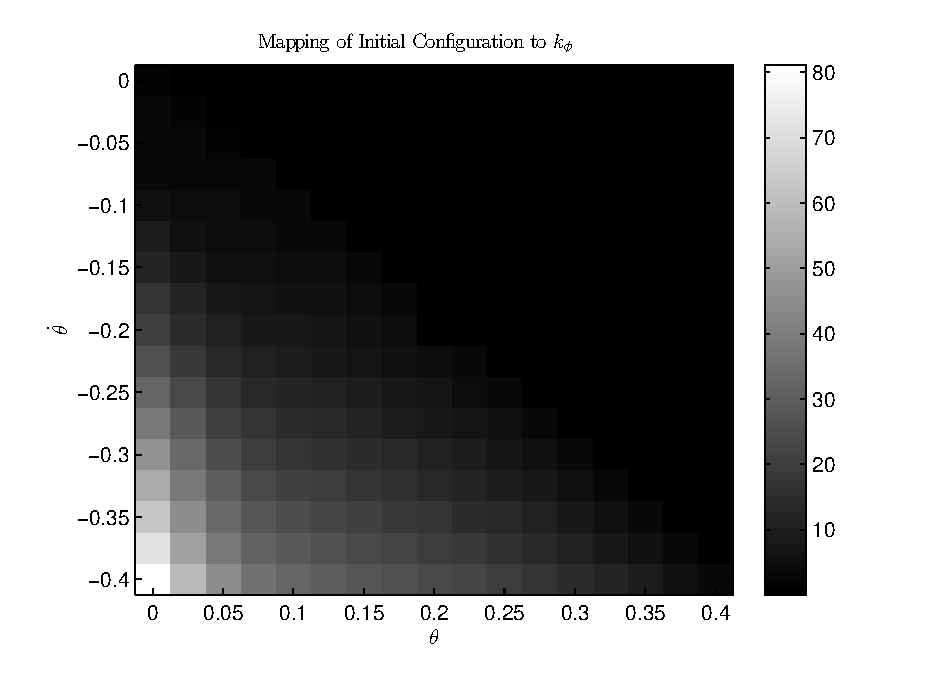
\includegraphics[scale=0.9]{K_values_17x17}
  \caption{Search result for the mapping
    $k_{\phi}=M(\theta_0,\dot{\theta_0})$.}
\end{figure}


The resulting mapping $k_{\phi}=M(\theta_0,\dot{\theta_0})$ is shown
in the figure \ref{fig:chp3-kvalues} for $\gamma=0.004$. As can be
seen, the mapping is monotonically increasing both as $\theta_0$
increases and as $\dot{\theta}_0$ decreases.

Before applying this mapping to an extended control policy for the
Simplest Biped Walking model implemented with a neuralfields-like
structure, a general architecture for neural field controllers is
presented.

\section{A Neural Field Controller Architecture}
\label{sec:chp3-neural}

In previous chapters it has been shown how a neural field can be used
as a controller for an unstable system. Neural fields have performed
good enough (compared to the RNN approach) when applied to a simple
control problem, a cart-and-pole (inverted pendulum) system. The
particular configuration tested was composed by:

*** This belongs to chp2 ***

\begin{itemize}
\item Two input variables: angular position and angular speed.
\item One control goal: to minimize the angular position.
\item One control action: lateral force at the pendulum base.
\end{itemize}

The corresponding controller architecture was devised as a two layer
neural field. Each layer of the field is actually a neural population
modeled after a subset of the real line: $x | x \in (-1,1)$.  Those
layers have the following roles:

\begin{itemize}
\item A first layer, without inner dynamics (i.e. not governed by a
  differential equation) which merely maps the input variables to
  activation potentials on a field, using the vector coding technique.
\item A second layer, with prototypical dynamics of neural fields. The
  kernel functions (for connections between layers 1 and 2, and for
  recurrent connections on layer 2) were used as the tuning/evolution
  parameters from which the control behavior emerged. The actual
  output was obtained by finding a weighted average of the activation
  potentials and mapping the resulting centroid to a single value (an
  inverse process to vector coding).
\end{itemize}

******

To generalize this approach, here is introduced a simple architecture
of neural field controllers to help the understanding of commonalities
and variations of the several controller structures developed next. It
is not meant as a global framework for control with neural fields, as
other architectures may be fruitfully developed. It is instead, an
specific model for the description of controllers based on layered
neural fields, able to describe the controller developed in this
chapter. The controller architecture that will be used here onwards is
described with an emphasis in how information is processed in the
controller.

The neural field controller architecture will be generally structured
as follows. It will have three layers: one input layer, one
representation layer and one action layer. As a strongly layered
architecture, the connections are only allowed from contiguous layers,
in one direction. Thus, elements in one layer cannot receive inputs
from other elements except those in the immediately preceding layer
(with \emph{action layer} receiving from \emph{representation layer},
and \emph{representation layer} receiving from \emph{input layer}).

For the controller used in this chapter, only the representation layer
is composed of neural populations, in terms of structure and behavior
(i.e. is governed by the dynamic equations of neural fields). The
elements in the input layer have the structure, but not the behavior,
of neural populations, and include a mapping function from input
variables (here the state-variables of the controlled system) to the
activation potential of its neural population. Finally, each element
in the action layer consist only of a mapping function from the
activation potential of a processing layer population to the value of
an output variable.

The layers are further described below:

\paragraph{Input Layer}
Each population on this layer is used as a spacial representation of a
function of the inputs. The values stored in the population act only
as a buffer to feed the inputs to the representation layer
populations, and correspond in each iteration to the mapping of an
input variable. While the mapping function can be general, here it
will be simplified. As a result, the input layer is a direct
representation of the relevant state of the controlled system (where
relevant means related to the control goal). It should be noted that
this layer is not governed by a differential equation and therefore
does not follow Amari's definition of a neural field.

For an input variable $e_i(t') \in \mathbb{R}^N$, the input mapping
function of input layer population $i$, assigns a potential
$u_i(\theta,t) \in \mathbb{R}$ to each position $x \in \mathbb{R}^N$
in the input layer population, at the current time $t$.

\begin{equation}
  \label{eq:eqn-inpos}
  u_i(x,t)=f_i(e_i(t'))
\end{equation}

Note that the instantaneous value of $u_i(x,t)$ is a function of the
input variable $e_i(t')$ for $t' \in [0,t]$, and therefore the mapping
function may have access to the entire history of $e_i$. In the
simplest case, the mapping function will depend only on the current
value $e_i(t)$, as the case in the controller developed in this
chapter.

\paragraph{Processing Layer}
Neural populations in this layer behave according to a differential
equation where the inputs are the functions of the potentials of
populations (for simplicity it will be assumed that only one
population in the preceding layer is an input to a given population,
and that input layer population is not shared among processing layer
populations). Therefore, those populations in this layer follow the
definition given by Amari for neural fields \cite{Amari}, but with an
specific structure for the interconnection between input layer and
processing layer populations.

The differential equation for the potential at position $x$ in a
population $j$ of the processing layer is:

\begin{align}
  \label{eq:lnf-oned}
  \tau_j\dot{u}_j(x,t)&=-u_j(x,t) +\int_{x' \in
    \Omega_j}{w_{j,j}\left( s_j(x,x') \right)
    \psi \left(u_j(x',t) \right) dx'} + S_j(x,t) \\
  S_j(x,t)&=\sum_{i \in \mathrm{In}}\int_{x' \in
    \Omega_i}{w_{i,j}\left(s_{i,j}(x,x') \right) \psi \left(u_i(x',t)
    \right) dx'}
\end{align}

Where as in previous chapters $\tau_j$ is a time constant for the
population $j$, $u_j$ is the activation potential of elements in the
population, $w_{i,j}$ is the connection kernel for connections from
population $i$ towards population $j$, which is a function of $s$, the
distance between two positions (on the same population $j$, or in
different populations $i$ and $j$), $X \in $In is a population in the
Input Layer, and $\psi$ is the activation function (usually a
Heaviside function, or a sigmoid).

The connection kernel $w_{i,j}$ may take any form, but the form of a
Mexican-hat function will be preferred.

In general, $x$ may be a position in any space (usually in
$\mathbb{R}$ or $\mathbb{R}^2$).

\paragraph{Output Layer}
This layer is used as a representation of the output values of the
controller architecture. As such, there will be one output population
for each output expected (or actuator controlled).

Similarly as it was done between the Input Layer and the Processing
Layer, the mapping between the Processing Layer and the Output Layer
is evaluated, for each output population, as the summation of the
transformation of each processing population. In other words, the
activation of an element located at $x$ in the output population $k$
is calculated as:

\begin{equation}
  \label{eq:eqn-outlayer}
  u_k(x,t)=\sum_{j \in \mathrm{Pr}}\alpha_{j,k}g_{j,k}(u_j(x',t))
\end{equation}

Where $\alpha_{j,k} \in [0,1]$ is a coefficient for the contribution
of each processing population on the output population, $j \in$ Pr is
a population in the processing layer, and $g_{j,Z}$ is the function
from the action potentials in the population $j$ to the resulting
contribution to the output population $k$ (before applying the
coefficient $\alpha$).

The function $g_{j,k}$ may take several forms. One possibility is to
perform a vector decoding (a reverse process that of the input
populations), calculated as an the centroid of the above defined
population potential. A more general function will be used for the
controller that is developed in this chapter.

\section{An Sliding-mode Neural Field Controller}
\label{sec:chp3-sliding}

The actual controller that is presented in this chapter, is an
instance of the neural field controller architecture defined above. It
is most closely related to Sliding-mode controllers, and works (in
general terms) selecting a control policy for each step (providing as
output the parameter $k_{\phi}$), using as input the Poincar� section
$v_n=[\theta_n \dot{\theta}_n]^T$. The mapping $k_{\phi}=M([\theta_n
\dot{\theta_n}]^T$ is embedded in the structure of the neural
field. The controller structure is detailed next.

The input layer contains two populations, one for $\theta_n$ and
another for $\dot{\theta_n}$, the elements in the Poincar� section
$v_n$. For these populations, the function $f$ in the equation
$u_i(x,t)=f(e_i(t'))$ performs a vector coding, i.e. an specific value
of the input variable $e_i$ causes an activation $u_i(x)$ with
amplitude 1 at some position $x$, and an activation of 0 at any other
position. For implementation purposes, there is a finite number of
elements, so the vector coding performed contributes to the two most
closely matched positions $x_a$ and $x_b$, so that
$u(x_a)x_a+u(x_b)x_b=e_i$.

The processing layer has one population, where the position $x$
resides in a two-dimensional euclidean space, defined as the subset of
$\mathbb{R}^2$ delimited by [0,0.4] x [-0.4,0]. An activation of an
element of an input population (e.g the one corresponding to
$\theta_n$) causes an activation that is reaches its maximum at some
row of elements in the processing layer, and decreases as the row are
father away. Likewise, an activation of an element in the other input
population, causes an activation peaking at some column. This
configuration gives the processing population an structure that
resembles the Poincar� section space. In the steady-state response,
the centroid of the population activation should correspond to the
Poincar� section vector $v_n$. The implementation has 17x17 elements,
an equal number than that of the mapping found in the section
\ref{sec:chp3-searching}.

The output layer has also one population, actually with only one
element, which activation provides the output value $k_{\phi}$. Each
element in the processing population contributes with a value given by
the product of the activation and the optimal $k_{\phi}$ value for
that position in the Poincar� section. The total output is calculated
as the weighted average:

\begin{align}
  u_{out}(x,t)&=g(u_{proc}(x',t)) \\
  g(u_{proc}) &= \frac{u_{proc}(x,t)M([\hat{\theta_n}
    \hat{\dot{\theta}_n}]^T=x)}{\int_{x' \in \Omega_{proc}}u_{proc}(x',t)dx'}
\end{align}


\section{Experimental Results}
\label{sec:chp3-results}
The experimental results are shown in the figures. For comparison
purposes, the State-feedback (SF) control strategy proposed by Wisse
et al. is implemented, and put side to side to the Sliding-mode(-like)
Neural Field controller (SMNF), as proposed in this chapter. The
experiment shown is run for $t=[0, 100]$ with initial configuration
$v_n=[0.02 -0.39]^T$, which is near the most unstable point in the
region studied.

While the SF controller. keeps constant the $k_{\phi}=100$ value in
order to attain stability, the SMNF controller proposed recalculates
the $k_{\phi}$ on each step using the current Poincar� section and the
embedded mapping $k_{\phi}=M(v_n)$. As the output value of the neural
field uses a centroid policy, it interpolates between the values on
the 17x17 mapping grid. This interpolation could potentially cause the
loss of stability (because the linear interpolation could underestimate
the required $k_{\phi}$, therefore a displacement
$k_{\phi}=M(v_n+[0.5h -0.5h]^T)$ in the mapping is applied,
guaranteeing stability given the monotonically increasing nature of
the mapping (where $h$ is the mapping grid step).

\begin{figure}[ht]
  \label{fig:figure1}
  \begin{minipage}[b]{0.5\linewidth}
    \centering
    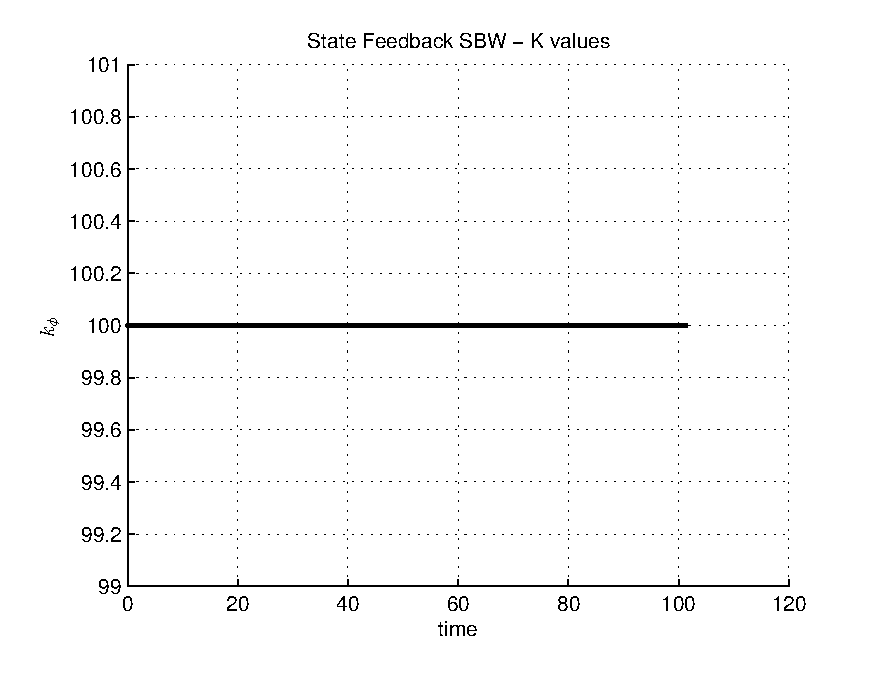
\includegraphics[scale=0.4]{SF_K}
    \caption{SF controller: $k_{\phi}$ vs time.}
  \end{minipage}
  \hspace{0.5cm}
  \begin{minipage}[b]{0.5\linewidth}
    \centering
    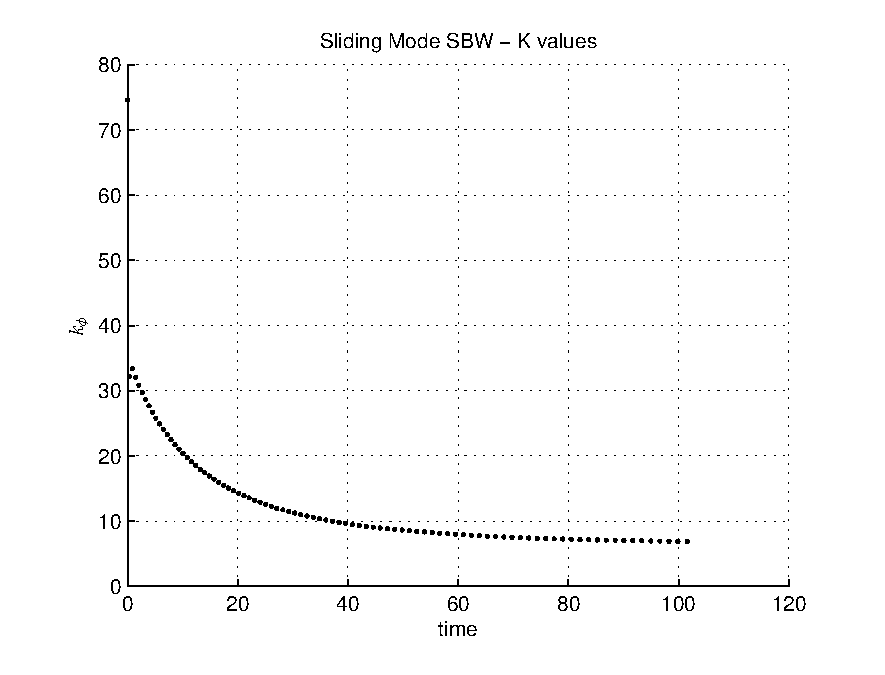
\includegraphics[scale=0.4]{SMNF2_K}
    \caption{SMNF controller: $k_{\phi}$ vs time.}
  \end{minipage}
\end{figure}

The overall performance of the SMNF controller is better than the SF
in terms of energy consumption and actuator strain, progressively
diminishing its $k_{\phi}$ value and thus the control action (see the
figure \ref{} where the K values vs time are plotted). The SF
controller converges faster to its fixed point (as would be expected
for a greater control action), but even in steady-state the control
action stays almost unaltered.

\begin{figure}[ht]
  \label{fig:figure1}
  \begin{minipage}[b]{0.5\linewidth}
    \centering
    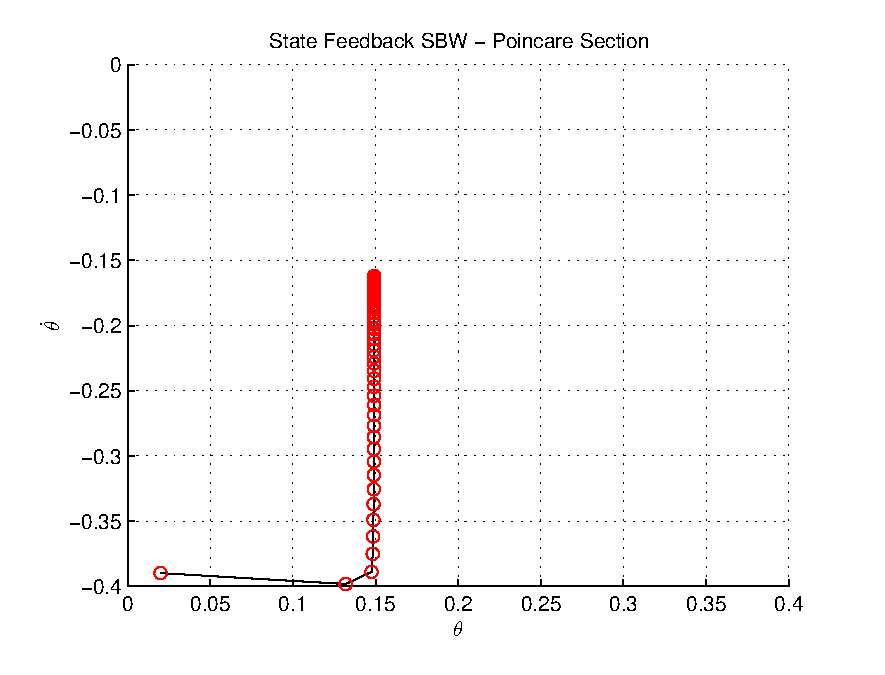
\includegraphics[scale=0.4]{SF_PS}
    \caption{SF controller: Poincar� Section.}
  \end{minipage}
  \hspace{0.5cm}
  \begin{minipage}[b]{0.5\linewidth}
    \centering
    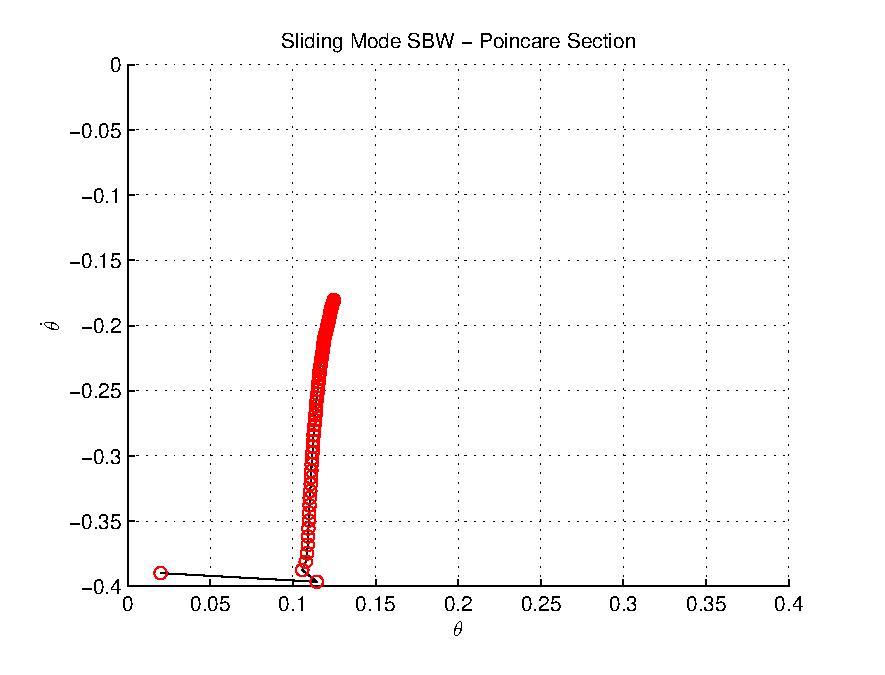
\includegraphics[scale=0.4]{SMNF2_PS}
    \caption{SMNF cont..: Poincar� Section.}
  \end{minipage}
\end{figure}

The Poincar� Section (see figure \ref{}) of the biped using the SMNF
controller shows how the system moves from a configuration that
requires higher $k_{\phi}$ values to configurations that require lower
ones, and that fact is exploited by the controller. The SF controller
also moves to configuration that require lower $k_{\phi}$ values (even
closer to the natural attraction basin of the biped), but that fact
remains unused.

\begin{figure}[ht]
  \label{fig:figure1}
  \centering
  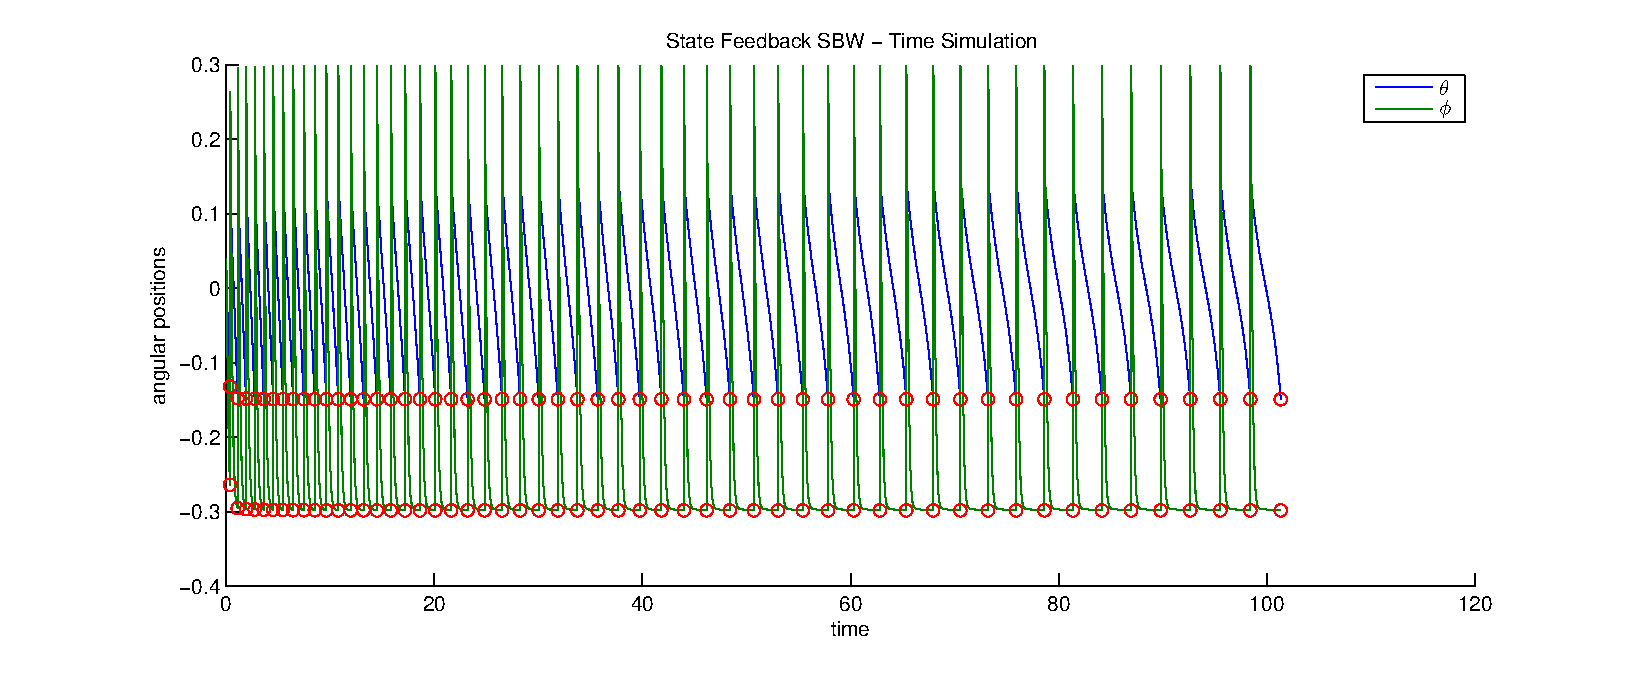
\includegraphics[scale=0.4]{SF_T}
  \caption{SF controller: Time simulation.}
\end{figure}

\begin{figure}[ht]
  \label{fig:figure1}
  \centering
  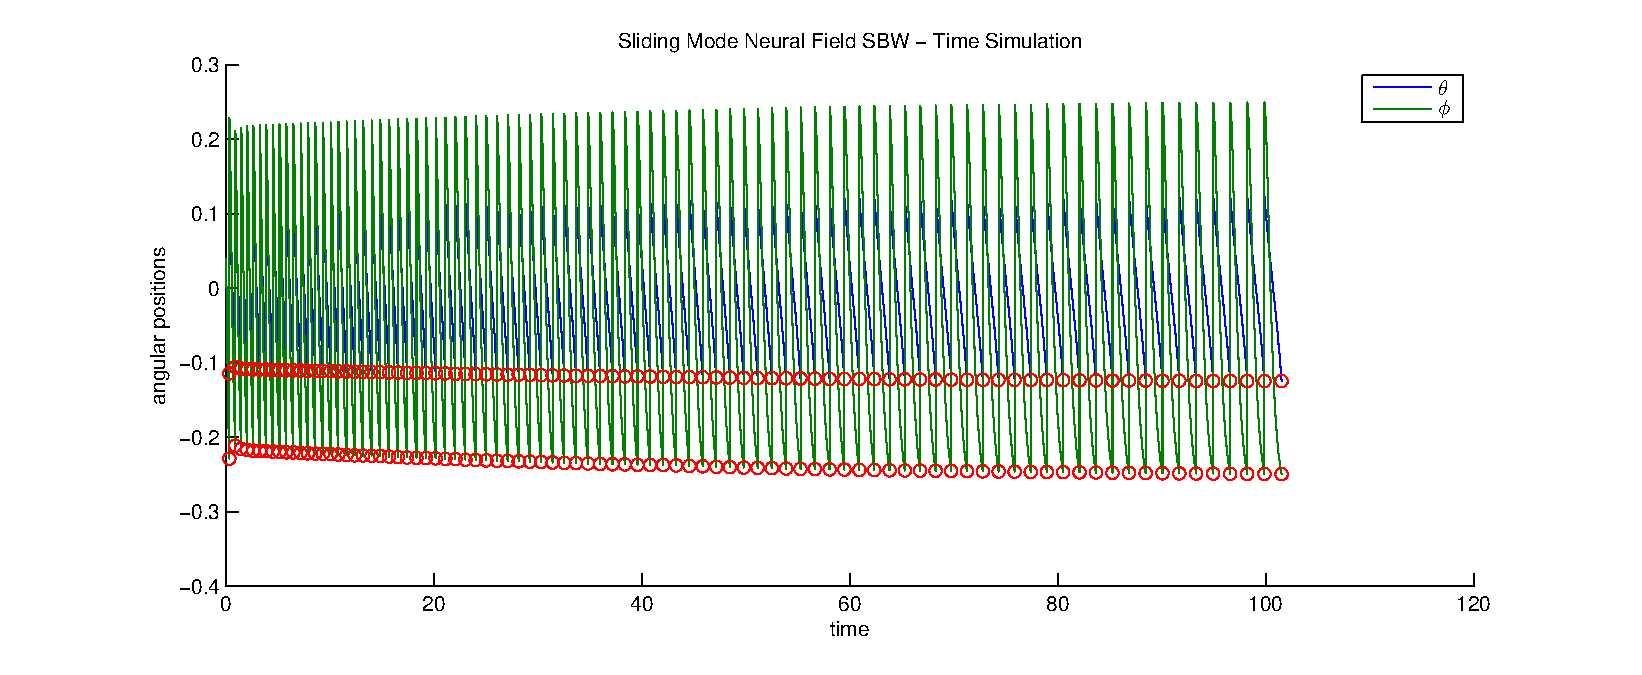
\includegraphics[scale=0.4]{SMNF2_T}
  \caption{SMNF controller: Time simulation.}
\end{figure}

The time simulation (see figure \ref{}) shows how the SMNF changes the
control policy (as parametrized by $k_{\phi}$) softly enough to
provide a qualitatively natural gait for the biped. It should be noted
that sudden changes of behavior are common in Sliding-mode
controllers, but that is mitigated in this case by three facts: 1) The
neural field applies an interpolation using the centroid of activation
to calculate the output $k_{\phi}$. 2) The neural field has natural
dynamics qualitatively equal to a low-band filter. 3) The change in
the $k_{\phi}$ occur at a non-linear point in the biped dynamics that
anyway would cause a jump in its state.

\section{Discussion}
\label{sec:chp3-discussion}
**TBD**

%%% Local Variables: 
%%% mode: latex
%%% TeX-master: "thesis"
%%% End: 

